%!TEX root = thesis.tex
\chapter{Methodology}
\label{c:methodology}
	


	This chapter describes the methodology used to find the optimum configurations of the ASF. In general terms, the optimum configuration must correspond to the following optimisation problem that has to be solved for PV modules as adaptive building shading systems:\\
	\begin{equation}
			minimise(C+H+L-PV)
	      	\label{e:minimise}
	\end{equation}

	Where $C$ is the electricity needed for cooling, $H$ is the electricty used for heating, $L$ is the lighting power demand and $PV$ represents the electricity production. \\
	An evaluation of the tools that were selected and how they are combined to create a modelling framework is given, and details of the simulation methodology are described.

	\section{Simulation Tool Selection}

		%In order to create an efficient simulation framework, various tools needed to be asessed. The general problem can be split up into

		To study the electricity generation and building energy consumption, a 3D geometry of the room and solar facade is built using the Rhinoceros software \cite{Rhino}, and its parametric modelling plugin Grasshopper \cite{grasshopper}. Rhinoceros is a state of the art computer-aided design (CAD) software, which can be used to generate complex geometries, such as the ASF. Grasshopper on the other hand, provides a visual programming language with a wide range of add-ons, detailed in Sections \ref{ss:buildEsim} and \ref{ss:radSim}. It is therefore particularly suited for simulations that are evaluating geometric structures. The simulation can then be split up into three parts, namely \emph{building energy simulations}, \emph{radiation simulations} and \emph{photovoltaic simulations}, which will be described in the following subsections. While Grasshopper is well suited for running simulations, it is not very suited for post-processing the data. The post-processing and optimisation was therefore done in Python, a programming language with powerful scientific packages, a simple syntax, extended documentation, and a very active community.  % In the following the corresponding tools are described. 

		%The aquired data is then post-processed in Python \cite{python} to extract the configurations that minimise building energy consumption and maximise PV electricity production.

		
		\subsection{Building Energy Simulation}
		\label{ss:buildEsim}

			 %The building energy simulation is conducted using EnergyPlus \cite{energyplus} through the DIVA \cite{DIVA} interface.
			There are various building energy analysis engines, such as EnergyPlus \cite{energyplus} or TRNSYS \cite{trnsys}. As EnergyPlus is open source, widely used, and well documented, it was chosen as the building simulation engine for all simulations within this thesis. There are multiple ways of connecting Grasshopper to EnergyPlus. Within this work, mainly DIVA \cite{DIVA} and Honeybee\cite{roudsari2014ladybug} were evaluated. While Honeybee provides a large range of settings and adaptability, its computational speed is significantly slower than DIVA. Therefore, and for its simplicity, DIVA was chosen to connect Grasshopper with EnergyPlus. In EnergyPlus, the geometric solar facade is interpreted as an external shading system. Simulations are performed for a whole year at fixed angle positions, outputting hourly values of energy use for heating, cooling and lighting. Optimum positions can then be found by comparing the electricity demand during every hour for all combinations. 
			%While Honeybee provides a large range of settings and adaptability, DIVA is kept very basic. However, the EnergyPlus analysis with honeybee is running significantly slower than with DIVA. Therefore, and for its simplicity, DIVA was chosen to connect Grasshopper with EnergyPlus. 

		\subsection{Radiation Simulation} 
		\label{ss:radSim}

			A solar radiance simulation is run using Ladybug \cite{roudsari2014ladybug}, which is another Grasshopper plugin. It includes various components to process weather data and calculate radiation on surfaces based on an automatically generated or a predefined mesh. Ladybug uses Radiance \cite{ward1994radiance} to determine the incident insolation on the solar facade. This approach enables the calculation of solar irradiance on the modules with high spatial resolution including the effect of module mutual shading as seen in Figure \ref{fig:radiation}. The radiation is analysed for cumulative monthly hours for the whole year. 

			\begin{figure}[H]
			\begin{center}
				%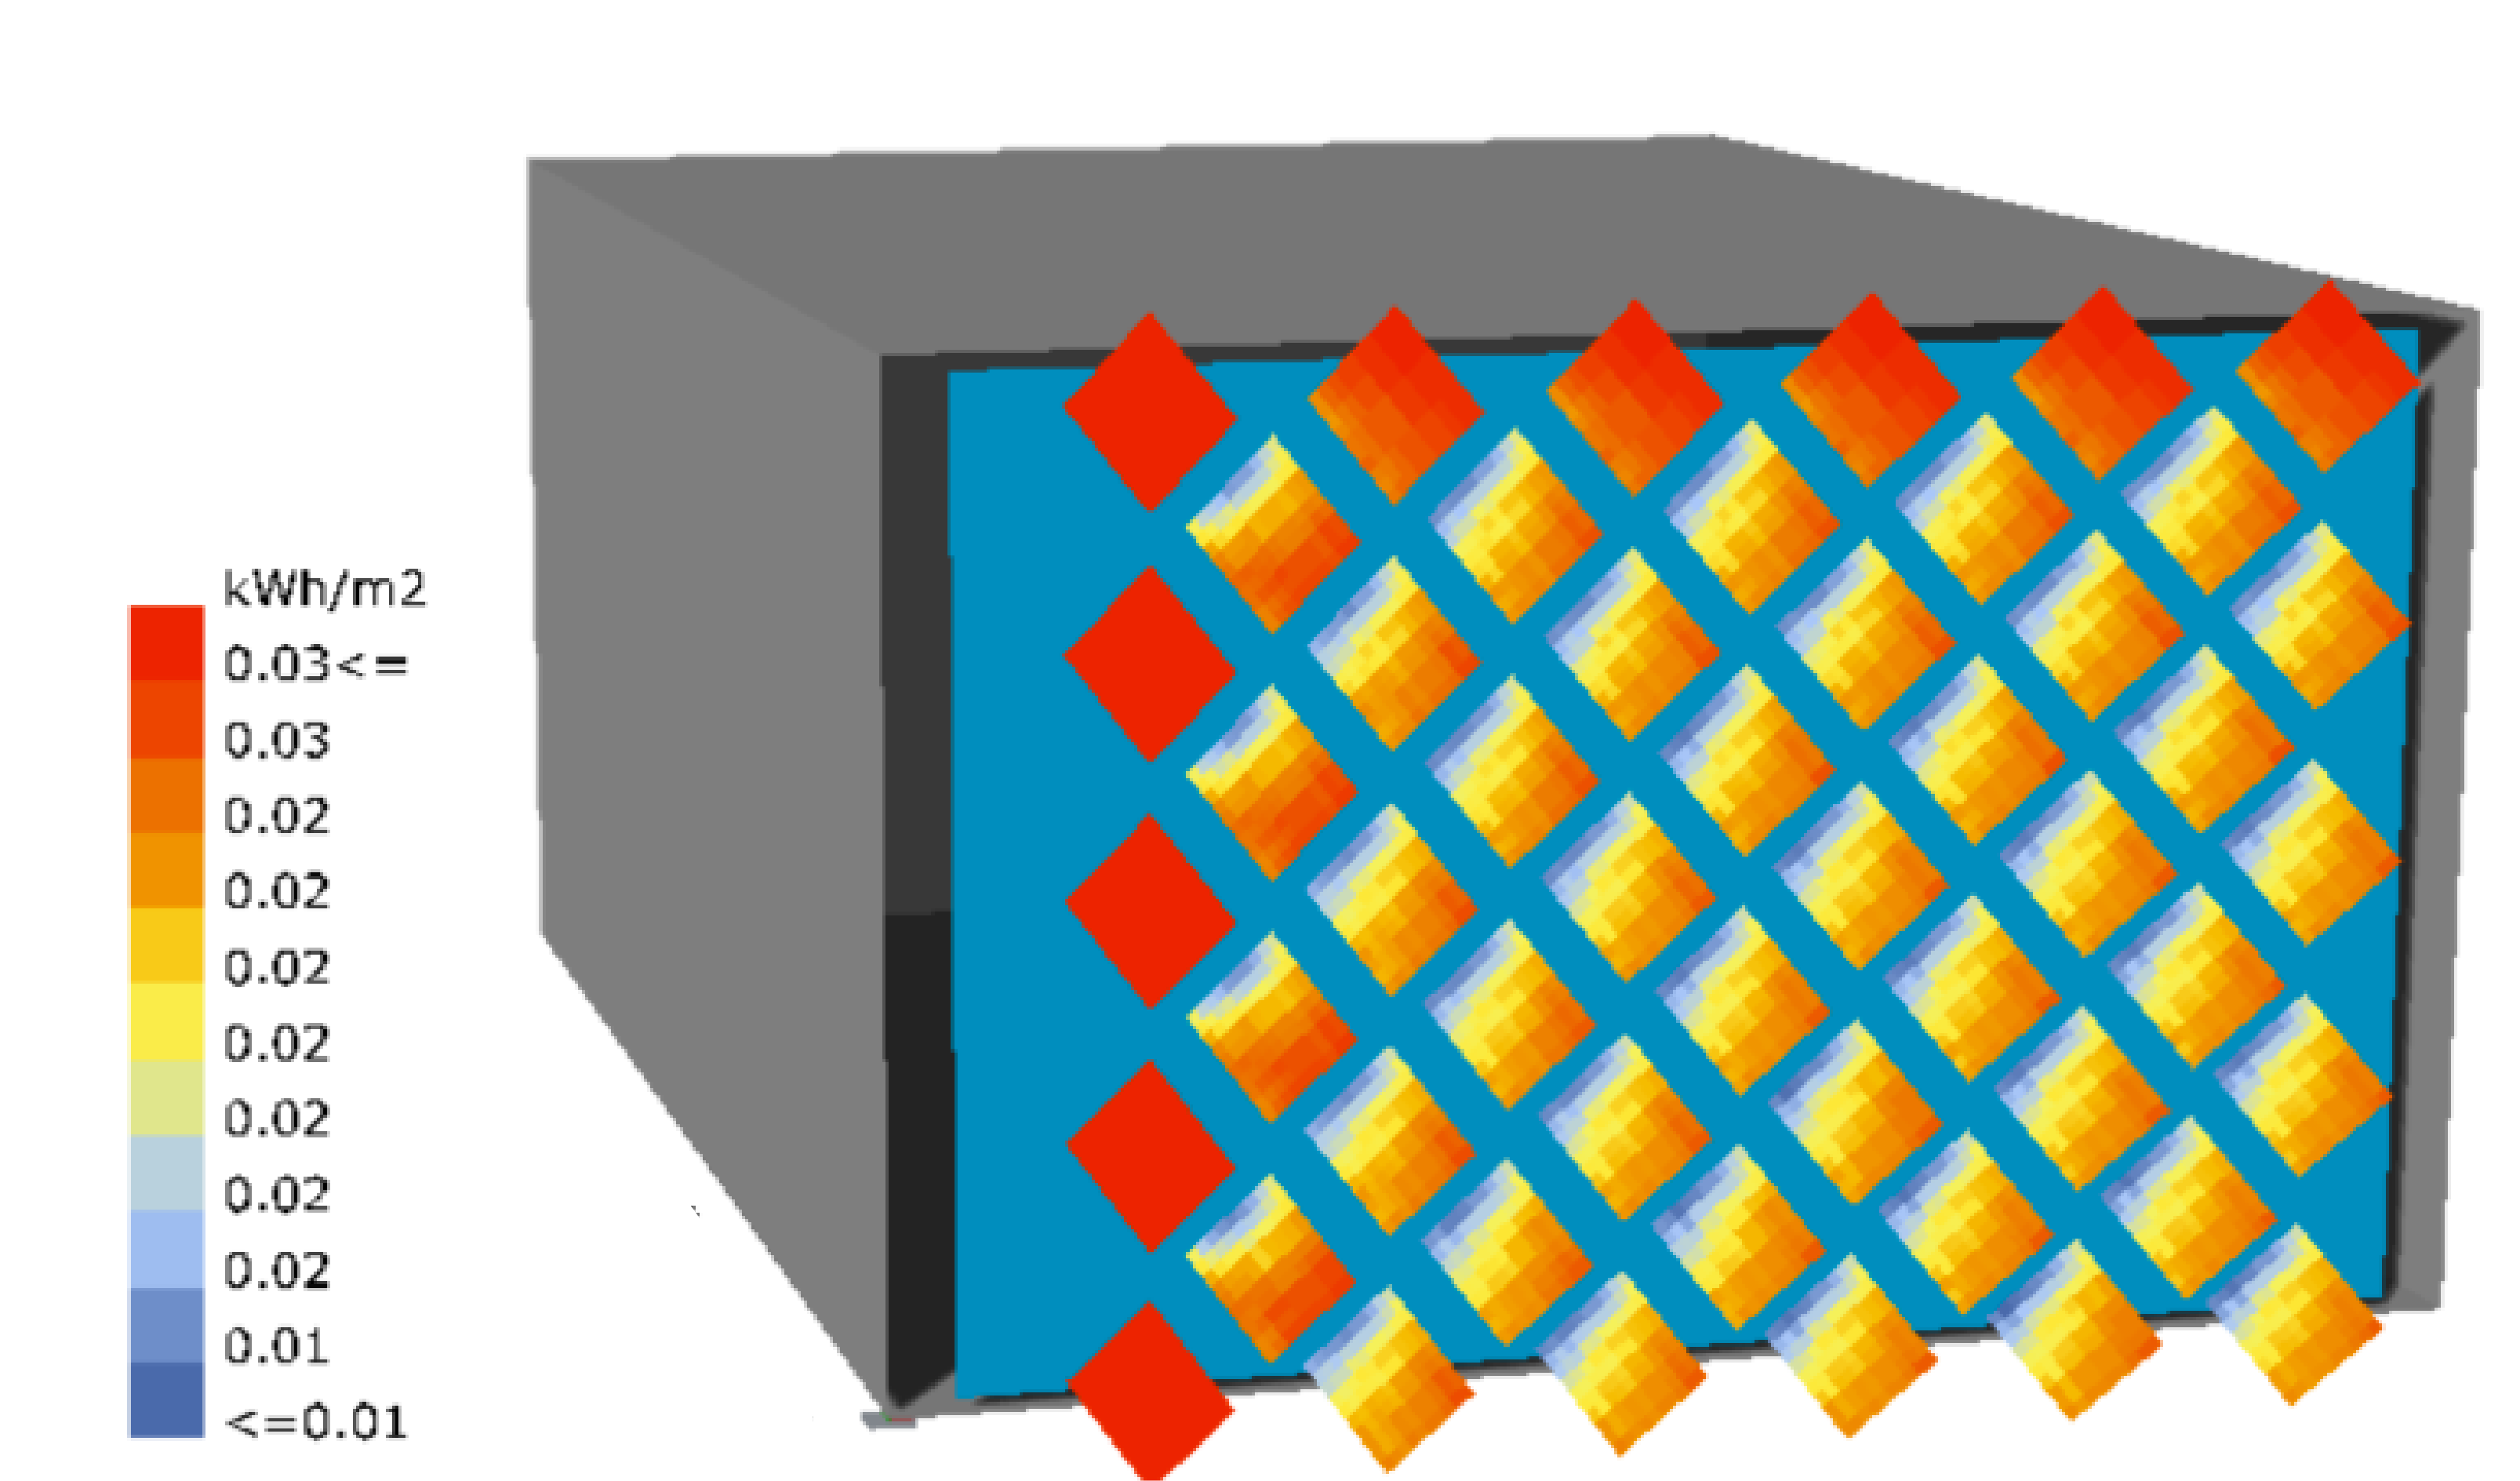
\includegraphics[width=8cm, trim= 0cm 0cm 0cm 0cm,clip]{radiationanalysis.png}Radiation_Results_aug11_1200_1300
				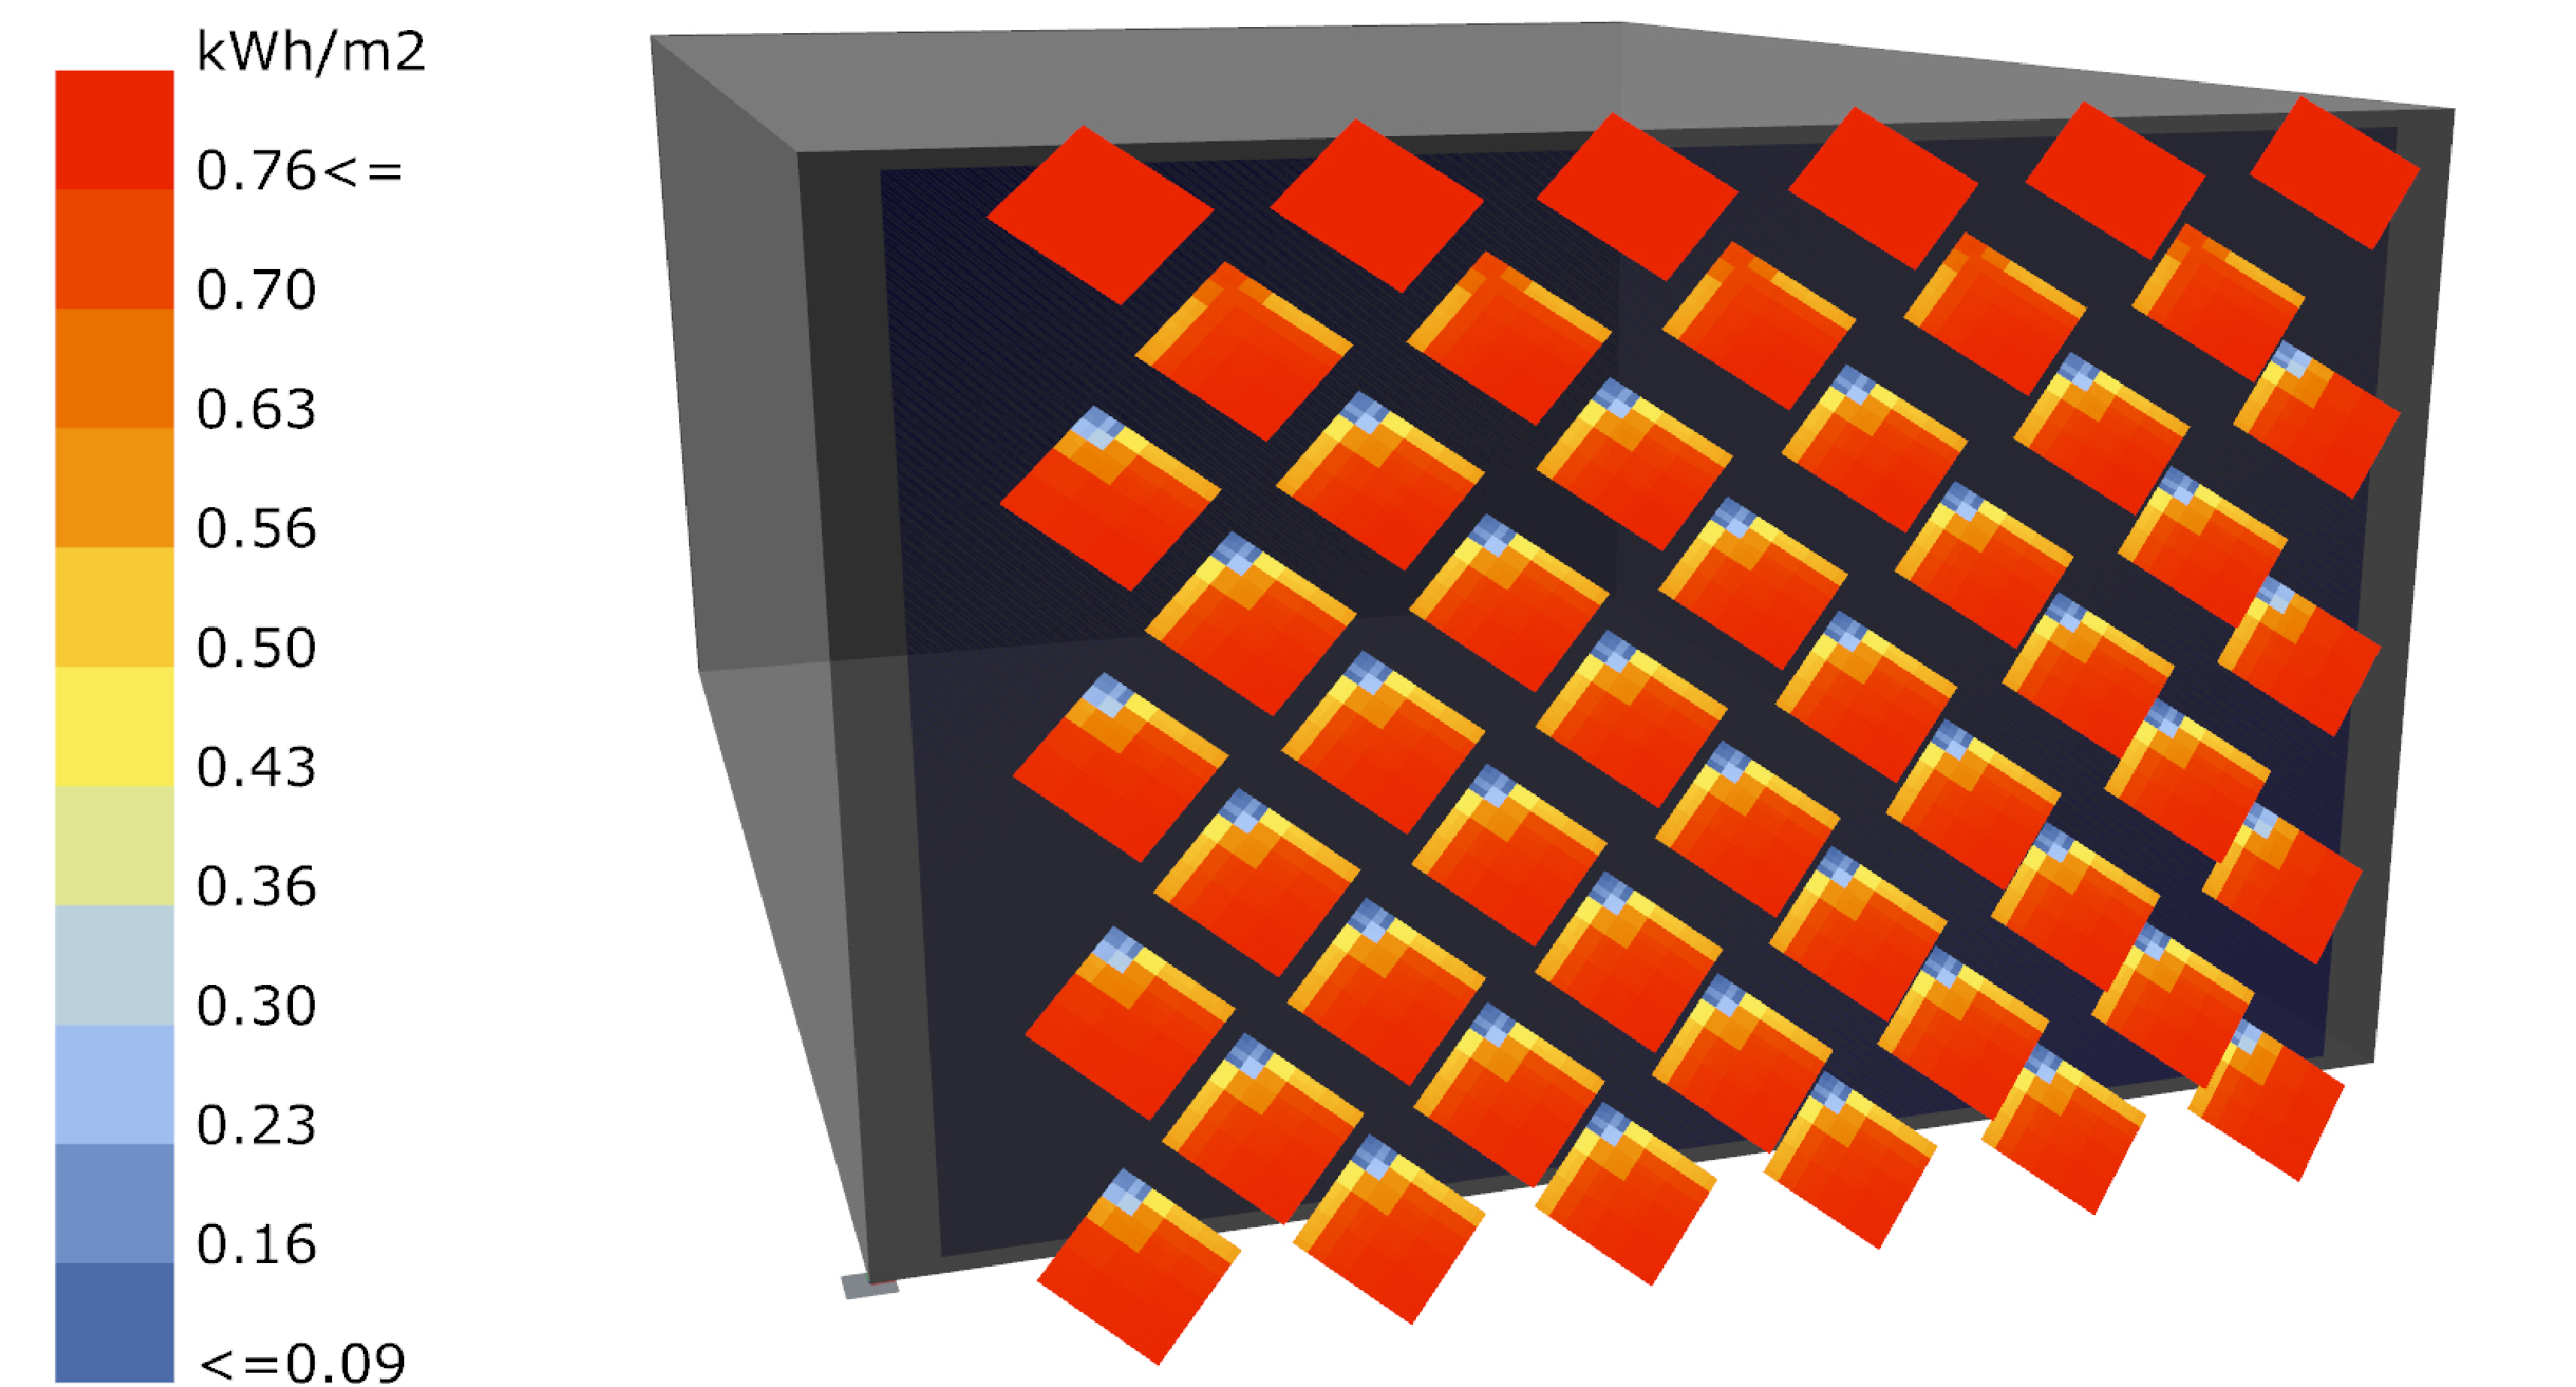
\includegraphics[width=\textwidth, trim= 0cm 0cm 0cm 0cm,clip]{Radiation_Results_aug11_1200_1300}
				\caption{A simulation result showing module insolation from 12:00-13:00 on the 11th of August for a weather file of Kloten-Zurich and a specific module orientation.}
				\label{fig:radiation}
			\end{center}
			\end{figure}

			\subsubsection{Grid Convergence}
			\label{ss:gridconvergence}

				%With a larger grid-size, radiation results are less accurate. In order to account for this effect, a grid convergence study was conducted. 
				A grid convergence study was conducted to determine the effect of the grid-size on the accuracy of the radiation results, as larger grid-sizes yield faster computational speeds, but generally at the cost of lower accuracy. Figure \ref{f:gridConvergence} shows the grid size dependency of the total radiation on the ASF. The colours in the first two plots on the upper left ((a) and (b)) represent the hours of the day. One can see in the second plot (b), where the radiation is normalized to the results when the grid-size is 12.5\,mm, that the simulations are significantly more accurate for morning and evening hours. This is caused by increased self-shading at midday hours. The colours in the third plot on the left (c) show the dependency on different combinations. No clear pattern could be found here. Finally, the average deviation is depicted in the fourth plot on the left (d) and a box-plot with all deviations is shown on the right (e). It can be seen that a smaller grid-size leads to larger deviations. While for a grid-size of 400\,mm the average deviation is over 10\%, the deviation goes down to below 1\% for a grid size of 25\,mm. 25\,mm was therefore taken as the grid-size of all simulations, as it gives accurate results, while still being computationally feasible. 

				\begin{figure*}
					\begin{center}
					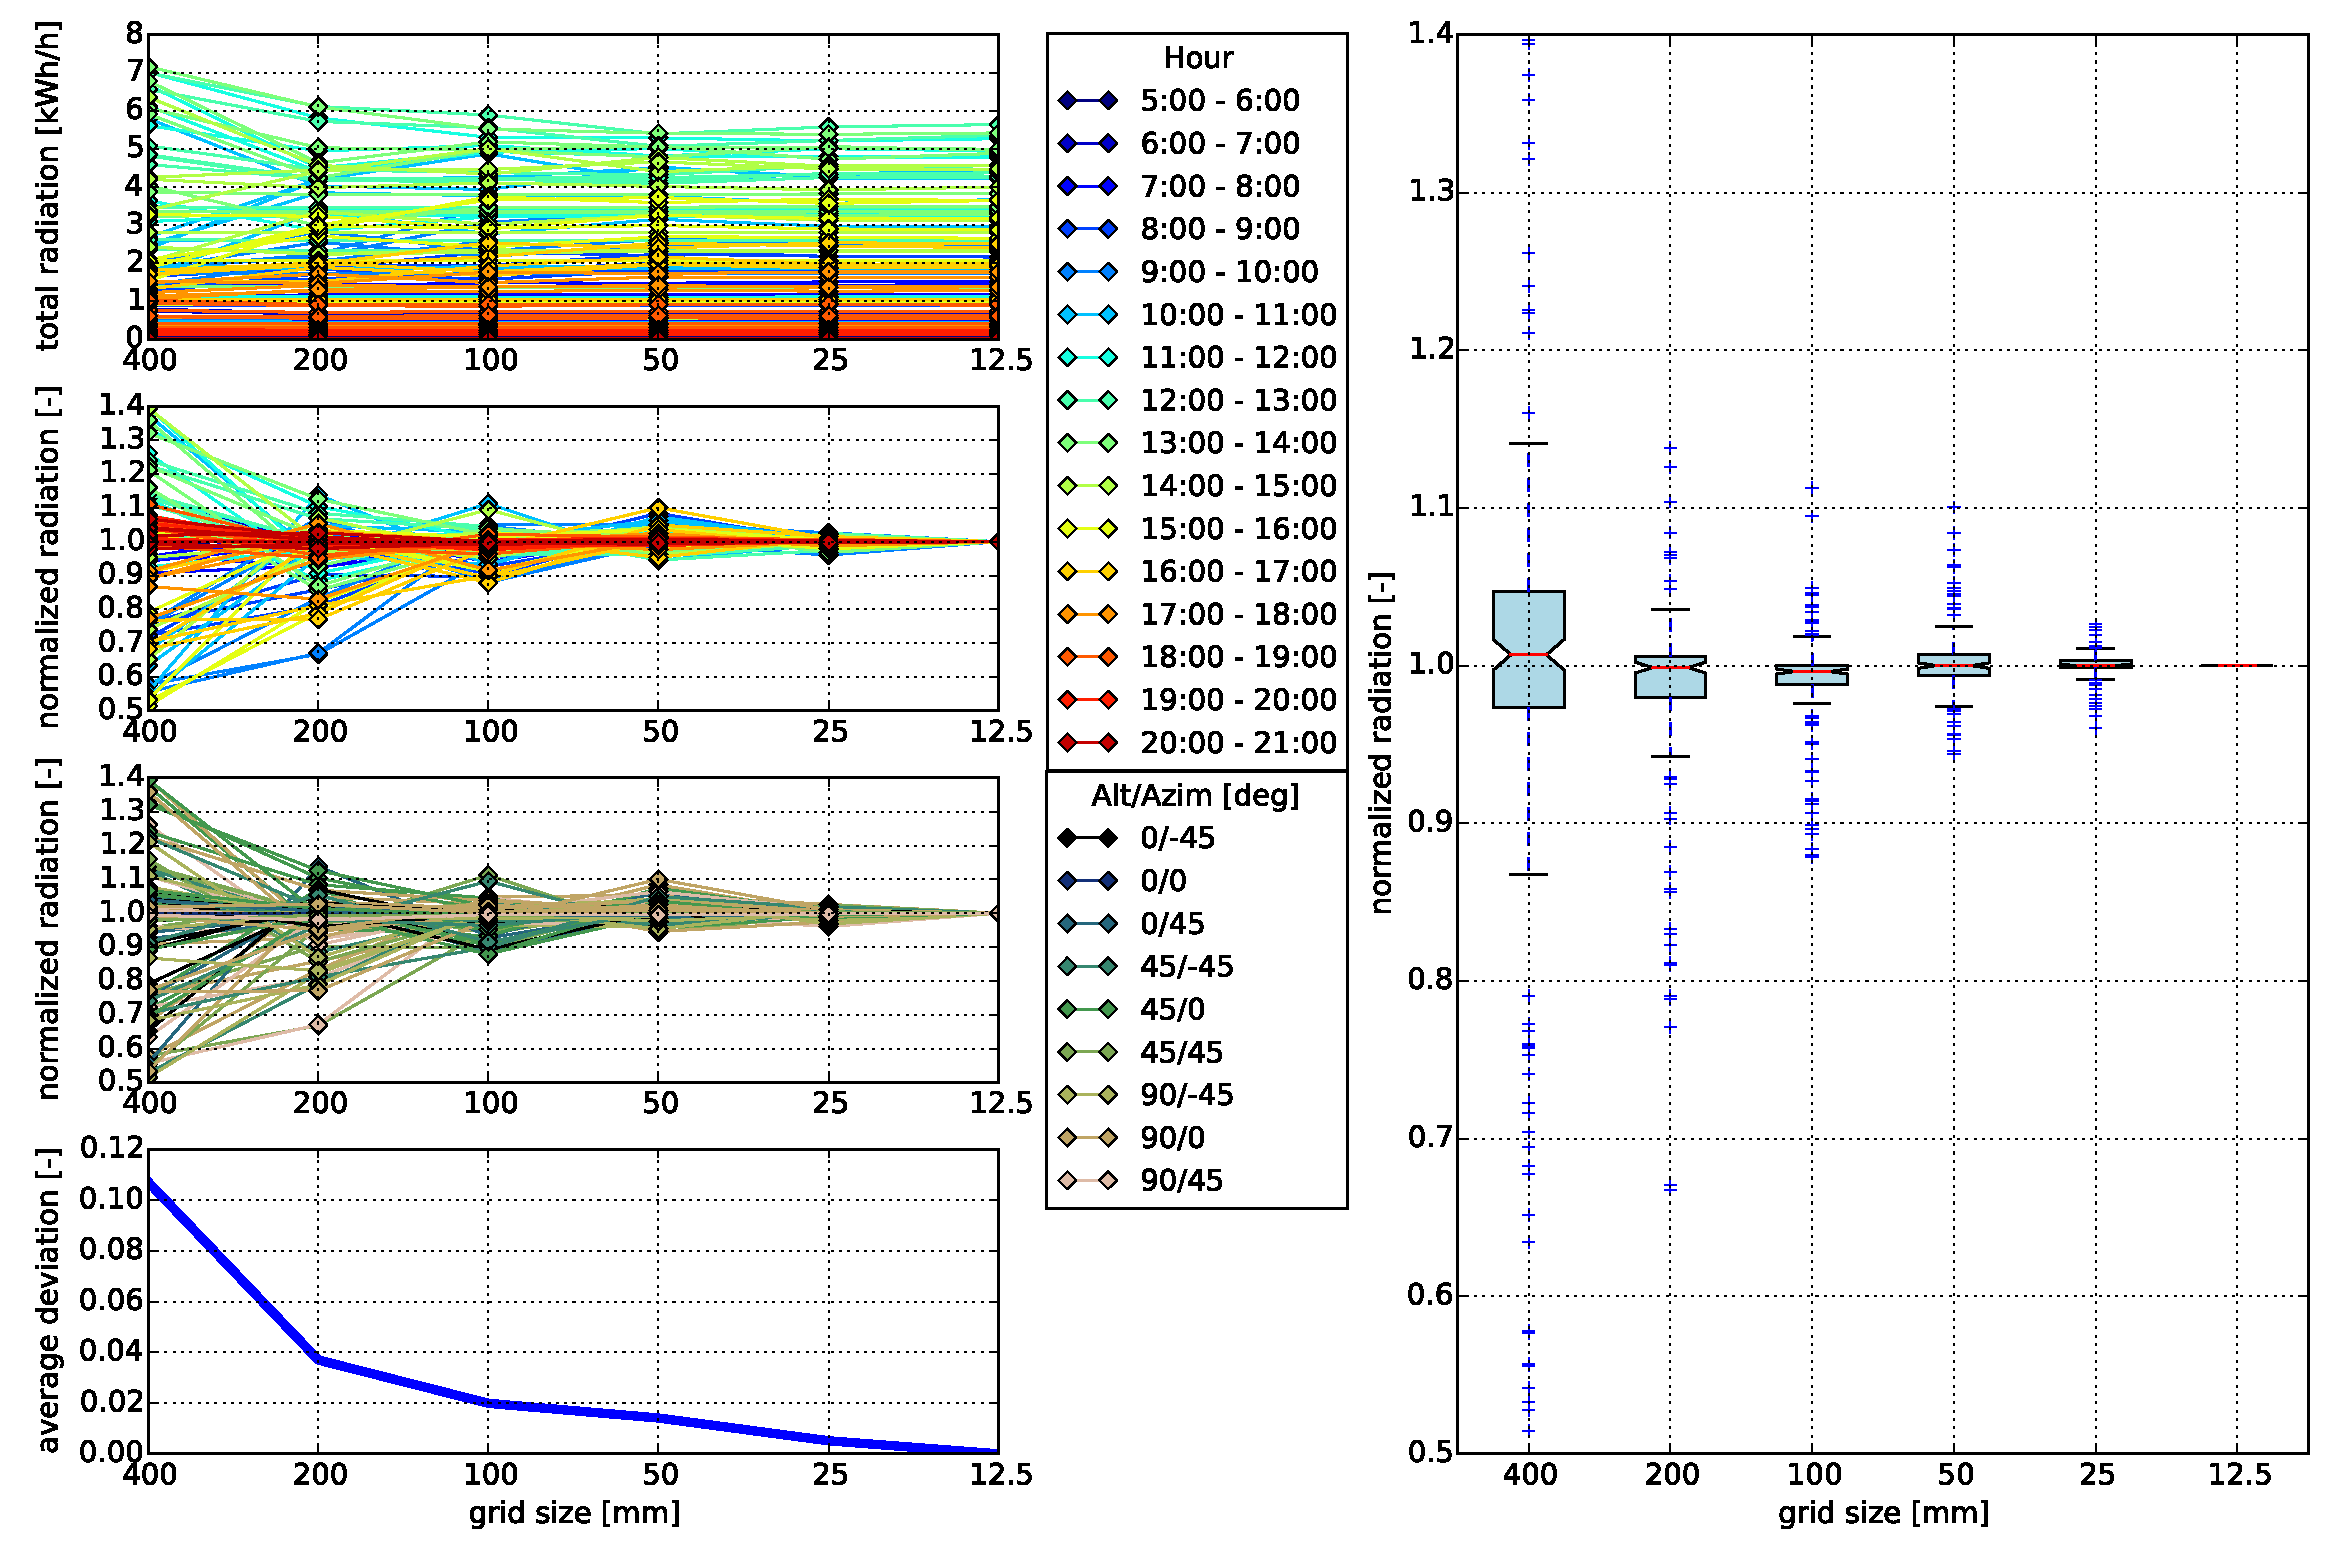
\includegraphics[width=\textwidth, trim= 0cm 0cm 0cm 0cm,clip]{gridConvergence.pdf}
					\caption{Grid convergence evaluation, showing the deviations of the radiation in dependence of the grid size, time of the day and panel orientation. (a) shows the total radiation on the panels in dependence of the hour of the day, (b) depicts the same results, but normalized with a division of the results with the smallest grid-size, (c) presents the influence of the panel orientation, (d) plots the average deviation from the smallest grid-size and (e) visualises all deviations with the usage of box-plots.}
					\label{f:gridConvergence}
					\end{center}
				\end{figure*}

		\subsection{Photovoltaic Simulation}
			%The  results are afterwards coupled to an electrical circuit simulation of thin-film PV modules with sub-cell level representation \cite{hofer2016}. 
			The electrical model of the PV cells builds up on the methodology presented in \cite{hofer2016} which is using the standard equivalent circuit model to calculate sub-cell I-V curves with a single diode, one series and one shunt resistance \cite{mermoud2010}. For the work in \cite{hofer2016}, the PV simulation was implemented with MATLAB. For this work, the MATLAB code was adjusted to match the new radiation simulations and then translated to python, in which the rest of the framework is written (details in Section \ref{s:simulationFramework}). PV electricity production is calculated based on a reference module. In addition to the irradiation dependency, the PV simulation includes temperature dependency. The temperature is estimated as suggested in \cite{Ross_Smokler_1986} with the following equation:

			\begin{equation}
				T_{cell} = T_{air} + \left(\frac{T_{cell}^0-T_{air}^0}{S^0}\right)S_{cell}
	      		\label{e:temp}
			\end{equation}

			where $T_{cell}$ is the temperature of each grid point on the module, $T_{air}$ is the ambient temperature, $T_{cell}^0$ is the temperature of the cell at reference insolation $S^0=800\frac{W}{m^2}$ and reference air temperature $T_{air}^0=20\degree C$, and $S_{cell}$ is the insolation of each gridpoint in $\frac{W}{m^2}$. The value of $T_{cell}^0$ was estimated using thermal images of the solar facade and typical values given in \cite{Ross_Smokler_1986} to be $38\degree C$. 



	\section{Simulation Framework}
	\label{s:simulationFramework}
		In order to combine the single simulations, an evaluation framework was built with the use of Grasshopper and Python. In the following, details on how the combination was done and on the resulting parametric simulation model are given.

		\subsection{Combined Evaluation}

			%As the Building energy simulations are achieved by using DIVA, wheras a radiation analysis is done with LadyBug, both within Grasshopper for Rhino. The results are then fed into a python script, which calculates the electricity production based on the radiation results and the surrounding temperature and post processes the information to calculate energy demand and optimum configurations. A corresponding workflow can be seen in Figure \ref{fig:workflow}.

			As the building energy and the radiation simulations are done within Grasshopper, whereas the PV simulation is done within Python, a framework is necessary to easily combine the simulations. For this end, a folder structure was created to manage the files that are written both within Grasshopper and Python. There are two main files for the combined evaluation, one Grasshopper and one Python file. In the Grasshopper file, all the parameters can be set and the simulations can be started. After the building energy and the radiation simulations are finished, the corresponding results are read by Python, where the PV electricity production is calculated and the results are combined. The combination of the building energy analysis with the PV electricity results is done by cumulatively combining the building energy results to correspond to the PV analysis format. With this, the net energy usage of the room including the PV electricity production of the ASF can be given for monthly hours as described in equation \ref{e:minimise}. An overview of the corresponding work-flow can be seen in Figure \ref{fig:workflow}. 
			% to find the optimal configurations as well as the corresponding energy. To combine the results of the building energy and the pv analysis, the building energy results were cumulatively combined to correspond to the pv analyis format. With this, the net energy useage of the room including the PV electricity production of the ASF can be given for monthly hours as described in equation \ref{e:minimise}. The an overview of the workflow can be seen in Figure \ref{fig:workflow}. 

			\begin{figure}[ht] %h can be omitted for better page layout
				\begin{center}
				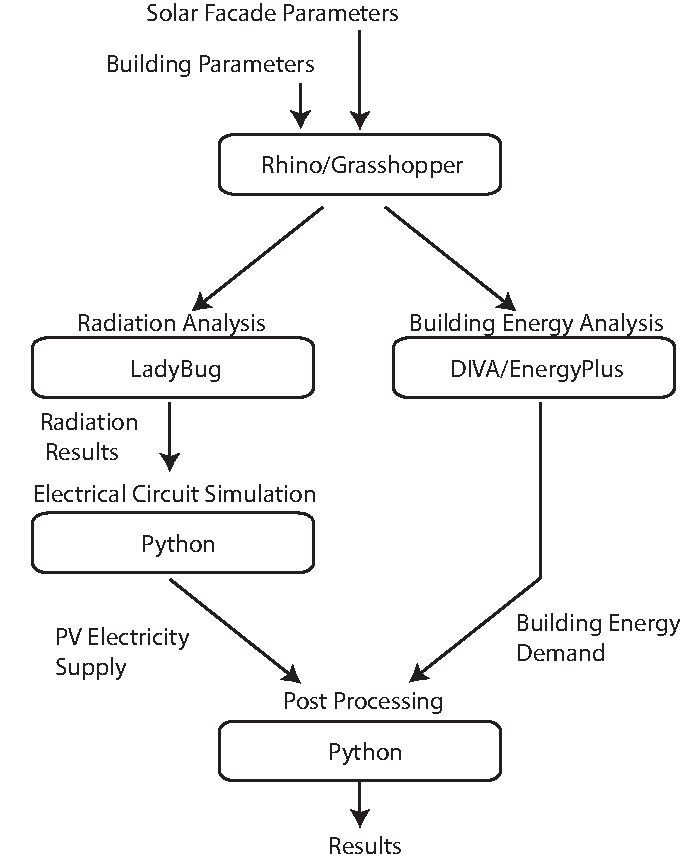
\includegraphics[width=0.75\textwidth, trim= 0cm 0cm 0cm 0cm,clip]{workflow_vertical}
				\caption{Work flow of the simulation framework}
				\label{fig:workflow}
				\end{center} 
			\end{figure}

			

		\subsection{Parametric Simulation Model}

			Because of the many influences on simulations, the evaluation environment was built as a parametric simulation model. The parameters that can be set and the outputs of the simulation model are shown in Figure \ref{fig:parametricModel}. The Location of the simulation is given by an epw weather file, out of which all relevant informations are automatically extracted. The building system can be varied according to the DIVA parameter inputs, that is heating and cooling COP, infiltration rate, lighting power, fresh air, material type and occupancy. The direction which the building and the facade are facing, can be set with a single number representing the deviation from south. Geometry settings are available for the ASF as well as for the building, enabling to easily evaluate every room size and facade layout. The actuation range is set by defining the azimuth and altitude angles, that will be evaluated. An additional input provides the possibility to split up the facade into multiple panel clusters, thus providing the possibility to account for the independent actuation of the panels. Finally, the radiation grid-size can be set, which influences accuracy of the radiation results and computational speed at the same time, as described in Section \ref{ss:gridconvergence}. 

			\begin{figure}[ht] %h can be omitted for better page layout
				\begin{center}
				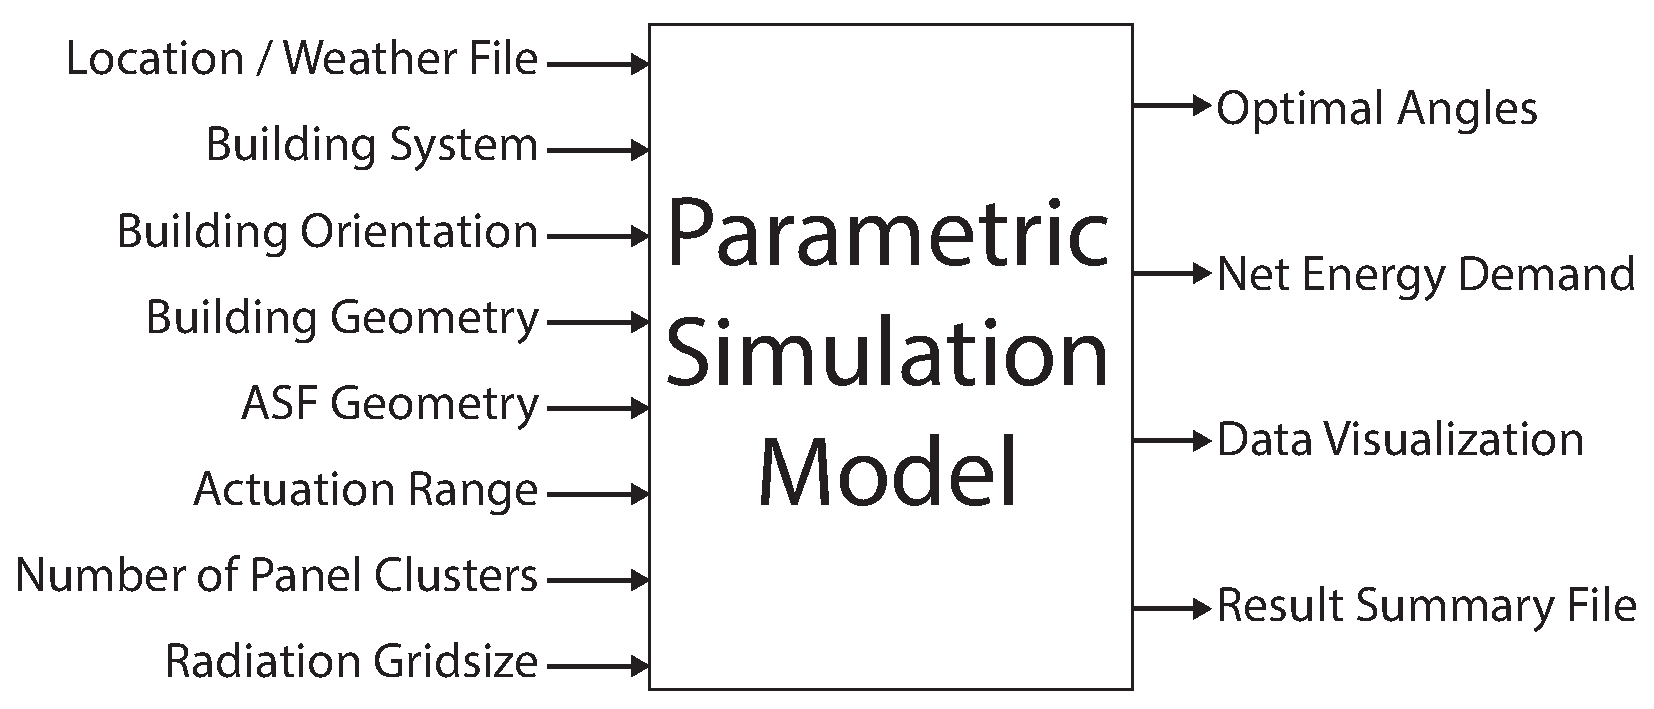
\includegraphics[width=\textwidth, trim= 0cm 0cm 0cm 0cm,clip]{parametricModel2}
				\caption{Blackbox visualization of the parametric simulation model}
				\label{fig:parametricModel}
				\end{center} 
			\end{figure}

	\section{Case Study}
		%The case study is done for a room and facade representing the prototype of the ASF at the house of natural resources (HONR) \cite{honr}.  The solar facade consists of 400mm CIGS square panels that can rotate in two degrees of freedom. On the horizontal axis, the panels can move from 0$^{\circ}$ (closed) to 90$^{\circ}$ (open) position in steps of 22.5$^{\circ}$. In the vertical axis, it can move from 45$^{\circ}$ to -45$^{\circ}$ in 22.5$^{\circ}$ steps. Existing ASF systems \cite{nagy2016} have independently actuated panels and a continuous range of actuation, however for simplicity, we group all panels into one cluster that moves in unison. This leaves us with 25 possible dynamic configurations of the facade system.

		The case study is done for a room and facade representing the prototype of the ASF at the house of natural resources (HONR) \cite{nagy2016}.  The solar facade consists of 400\,mm CIGS square panels that can rotate in two degrees of freedom. On the horizontal axis, the panels can move from 0$^{\circ}$ (closed) to 90$^{\circ}$ (open), whereas in the vertical axis, they can move from -45$^{\circ}$ to 45$^{\circ}$. %Existing ASF systems \cite{nagy2016} have independently actuated panels and a continuous range of actuation, however for simplicity, we group all panels into one cluster that moves in unison. This leaves us with 25 possible dynamic configurations of the facade system. 

		The office environment is heated with a heatpump with an average COP of 4 and cooled with an average COP of 3. When required, the electric lighting consumption is 11.7 $W/m^2$. 

		%A simulation of each possible dynamic configuration of the facade is run for each hourly timestep of the year using using a weather file for Kloten, Switzerland. %\cite{genevaweatherfile}. %The results are then post-processed in Python \cite{python} to extract the configurations that minimise building energy consumption and maximise PV electricity production.

		Simulations are run for different angle combinations, with a weather file for Kloten-Zurich, Switzerland. There are two base-cases for the simulations. The first one consists of 49 different angle combinations (i.e. seven azimuth and seven altitude angles, with a stepsize of $15\degree$), which is used for detailed evaluations of the angle positions. The second base-case consists of 25 angle combinations (five azimuth and five altitude angles), this case is used for the comparison of different system parameters. Simulations are done for average days of every month of the year, and the results are then compared to control strategies where the angles are fixed or follow sun tracking. Furthermore, the sensitivity of various parameters, such as building orientation, location, and COP of the heating/cooling system is evaluated. A corresponding picture of the prototype installed at the HONR, can be seen in Figure \ref{fig:honr}. 

		\begin{figure}[ht] %h can be omitted for better page layout
			\begin{center}
			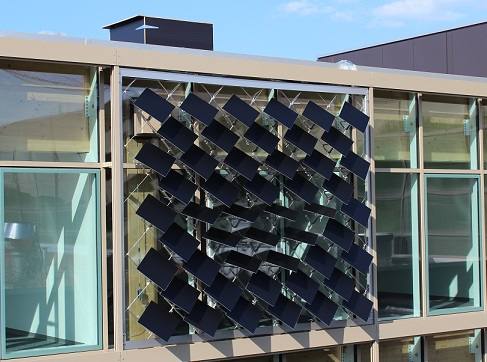
\includegraphics[width=0.75\textwidth, trim= 0cm 0cm 0cm 0cm,clip]{honr_small}
			\caption{Prototype of the adaptive solar facade on the house of natural resources}
			\label{fig:honr}
			\end{center} 
		\end{figure}



